\documentclass[11pt]{article}
\usepackage{multicol}
\usepackage{graphicx}
\usepackage{todonotes}
\usepackage{tcolorbox}

\usepackage{anysize,color,float,graphicx,url,comment,hyperref,ulem}
\usepackage{hyperref}
\hypersetup{
    colorlinks=true,
    linkcolor=blue,
    filecolor=magenta,      
    urlcolor=red,
}
\usepackage{amsmath, amsfonts, amssymb}
\usepackage{enumitem}
\usepackage{HW}
\includecomment{comment}
\excludecomment{studentSpace}
\includecomment{studentSpace}
\includecomment{answer}
\excludecomment{answer}
\includecomment{comment}
\newcommand{\blank}{
\underline{\hspace{1.5cm}\hspace{1.5cm}}
}
\newcommand{\norm}[1]{\left\lVert#1\right\rVert}

\begin{document}
\titleline{\semester}
\exhead{Problem Set: Due: 10:00 PM,  18-Feb}
\begin{itemize}
\item Please write (only if true) the honor code. If you used any
  source (person or thing) explicitly state it. 

\item Important: This is an INDIVIDUAL assignment.

\item Always provide a brief explanation. (The length of the
  explanation required has been forecasted with the amount of space
  provided.)
  
\item Submit following files in folder name lab03\_roll\_XX :
	\begin{enumerate}
      \item readme.txt (case sensitive name). This \emph{text} file
        contains identifying information, honor code, links to
        references used 
      \item ReflectionEssay.pdf is optional but a brief one would be nice.
      \item lab03\_roll\_XX.pdf (includes all solutions). 
      \item All relevant tex source (and images only if necessary). No
        other junk files, please.
     \end{enumerate}
\end{itemize} 

\hrulefill
\begin{enumerate}

\begin{tcolorbox}
\item  State whether or not the following points are the same and explain why.
\begin{multicols}{2}
\begin{enumerate}[]
\item
$A[2, -1, 3]$, $B[4,-2,6]$
\item
$A[\sqrt{2}/2, -1,0]$, $B[1,-\sqrt{2},0]$
\end{enumerate}
\end{multicols}
\begin{studentSpace}
Ans\\
a)Yes, both the points are same. Since in projective geomtery, scaling the coordinates by some factor doesn't change the point. A  A point is effectively a ray through origin if embedded in $R^{3}$. Here both points can be reduced to $(\frac{2}{3},\frac{-1}{3},1)$ point\\\\
b)The ideal points represent a direction in projective space. Both the shown coordinates have same direction with an angle of $\arctan(-\sqrt{2})$. Hence the given ideal points are same.
\vspace{3cm}
\end{studentSpace}

\end{tcolorbox} \begin{tcolorbox}
\item In projective three-space, what are the standard homogeneous
  coordinates of (a) the origin and (b) ideal points determined by the
  intersections of the extensions of the coordinate axes and the ideal
  plane?\\
Ans\\
a)The origin in $P^3$ space is 4 tuple = (0,0,0,1) \\\\
b) We know that all Ideal points lie on Ideal Plane given by (0,0,0,1). Now equation of X-axis can be found out by linear combination of 2 planes , specifically x-y plane and x-z plane. So we will get x-axis  = $\lambda(0,1,0,0) + \mu(0,0,1,0)$. Now to find intersection of x-axis with ideal plane, we can simply take the intersection of these three planes ((0,0,0,1),(0,1,0,0),(0,0,1,0)). This will be given by solving the 4 3x3 determinants, which will give us (1,0,0,0) as the intersection. Similarly intersection of y-axis with Ideal Plane will be (0,1,0,0) and intersection of z-axis with Ideal Plane will be (0,0,1,0).
\begin{studentSpace}
\vspace{1cm}
\end{studentSpace}
\end{tcolorbox}

\begin{tcolorbox}
\item Write standard homogeneous coordinates for the points specified
  in uppercase characters. (Use left and right to distinguish.)\\
Ans\\  
\textbf{Left:}\\ 
A = (-1.5,1),
B = (3,1),
C = (5,1),
D = (5.5,1),
E = (1,0)\\
\textbf{Right:}\\
A = (0,0,1),
B = (2,0,1),
C = (3,1,1),
D = (1,1,0),
E = (-1,4.5,1),
F = (-1,1,0),\\
G = (-3,4,1),
H = (-4,3,1),
I = (-1,1,1),
J = (-4,-2,1),
K = (1,-4,1),\\
L = (1.5,-0.5,1),
M = (0,-1,0)

\begin{studentSpace}
\vspace{3cm}
\end{studentSpace}



\end{tcolorbox} \begin{tcolorbox}
\item Which of the following points lie on the line $3p_1 -2p_2+5p_3 =
  0$?  Why?
\begin{multicols}{2}
\begin{enumerate}[]
\item
$A[1,1,2]$
\item
$B[4,1,-2]$
\end{enumerate}
\end{multicols}
\begin{studentSpace}
Ans\\
a) The dot product of point with line should be equal to 0 if point lies on line. The line is represented as (3,-2,5). We see that (1,1,2)$\cdot$(3,-2,5) = 11 $\neq$ 0. Hence point A doesn't lie on line.\\
b)The dot product of B with line is: (4,1,-2)$\cdot$(3,-2,5) = 0. Hence point B lies on the line.
\vspace{3cm}
\end{studentSpace}

\end{tcolorbox} \begin{tcolorbox}
\item Write the coordinates of the lines that are the extensions to the
  protective plane of the following Euclidean lines.
\begin{multicols}{2}
\begin{enumerate}[]
\item
$3x + 2y = 6$
\item
$4x + 5y + 7 = 0$
\end{enumerate}
\end{multicols}
\begin{studentSpace}
Ans\\
For converting to projective space, we simply replace x by $\frac{X}{Z}$ and y by $\frac{Y}{Z}$.\\
a) 3x + 2y -6 = 0 becomes 3X + 2Y -6Z = 0. Hence coordinates of the line become (3,2,-6).\\
b)4x + 5y + 7 = 0 becomes 4X + 5Y + 7Z = 0. Hence coordinates of the line become (4,5,7).
\vspace{3cm}
\end{studentSpace}

\end{tcolorbox} \begin{tcolorbox}
\item Sketch each line in the projective plane whose equation is given.
\begin{multicols}{2}
\begin{enumerate}[]
\item
$2p_1 + 3p_2 + 5p_3 = 0$
\item
$3p_1 - 2p_2 - p_3 = 0$
\end{enumerate}
\end{multicols}
\begin{studentSpace}
\begin{figure}[H]
    \centering
    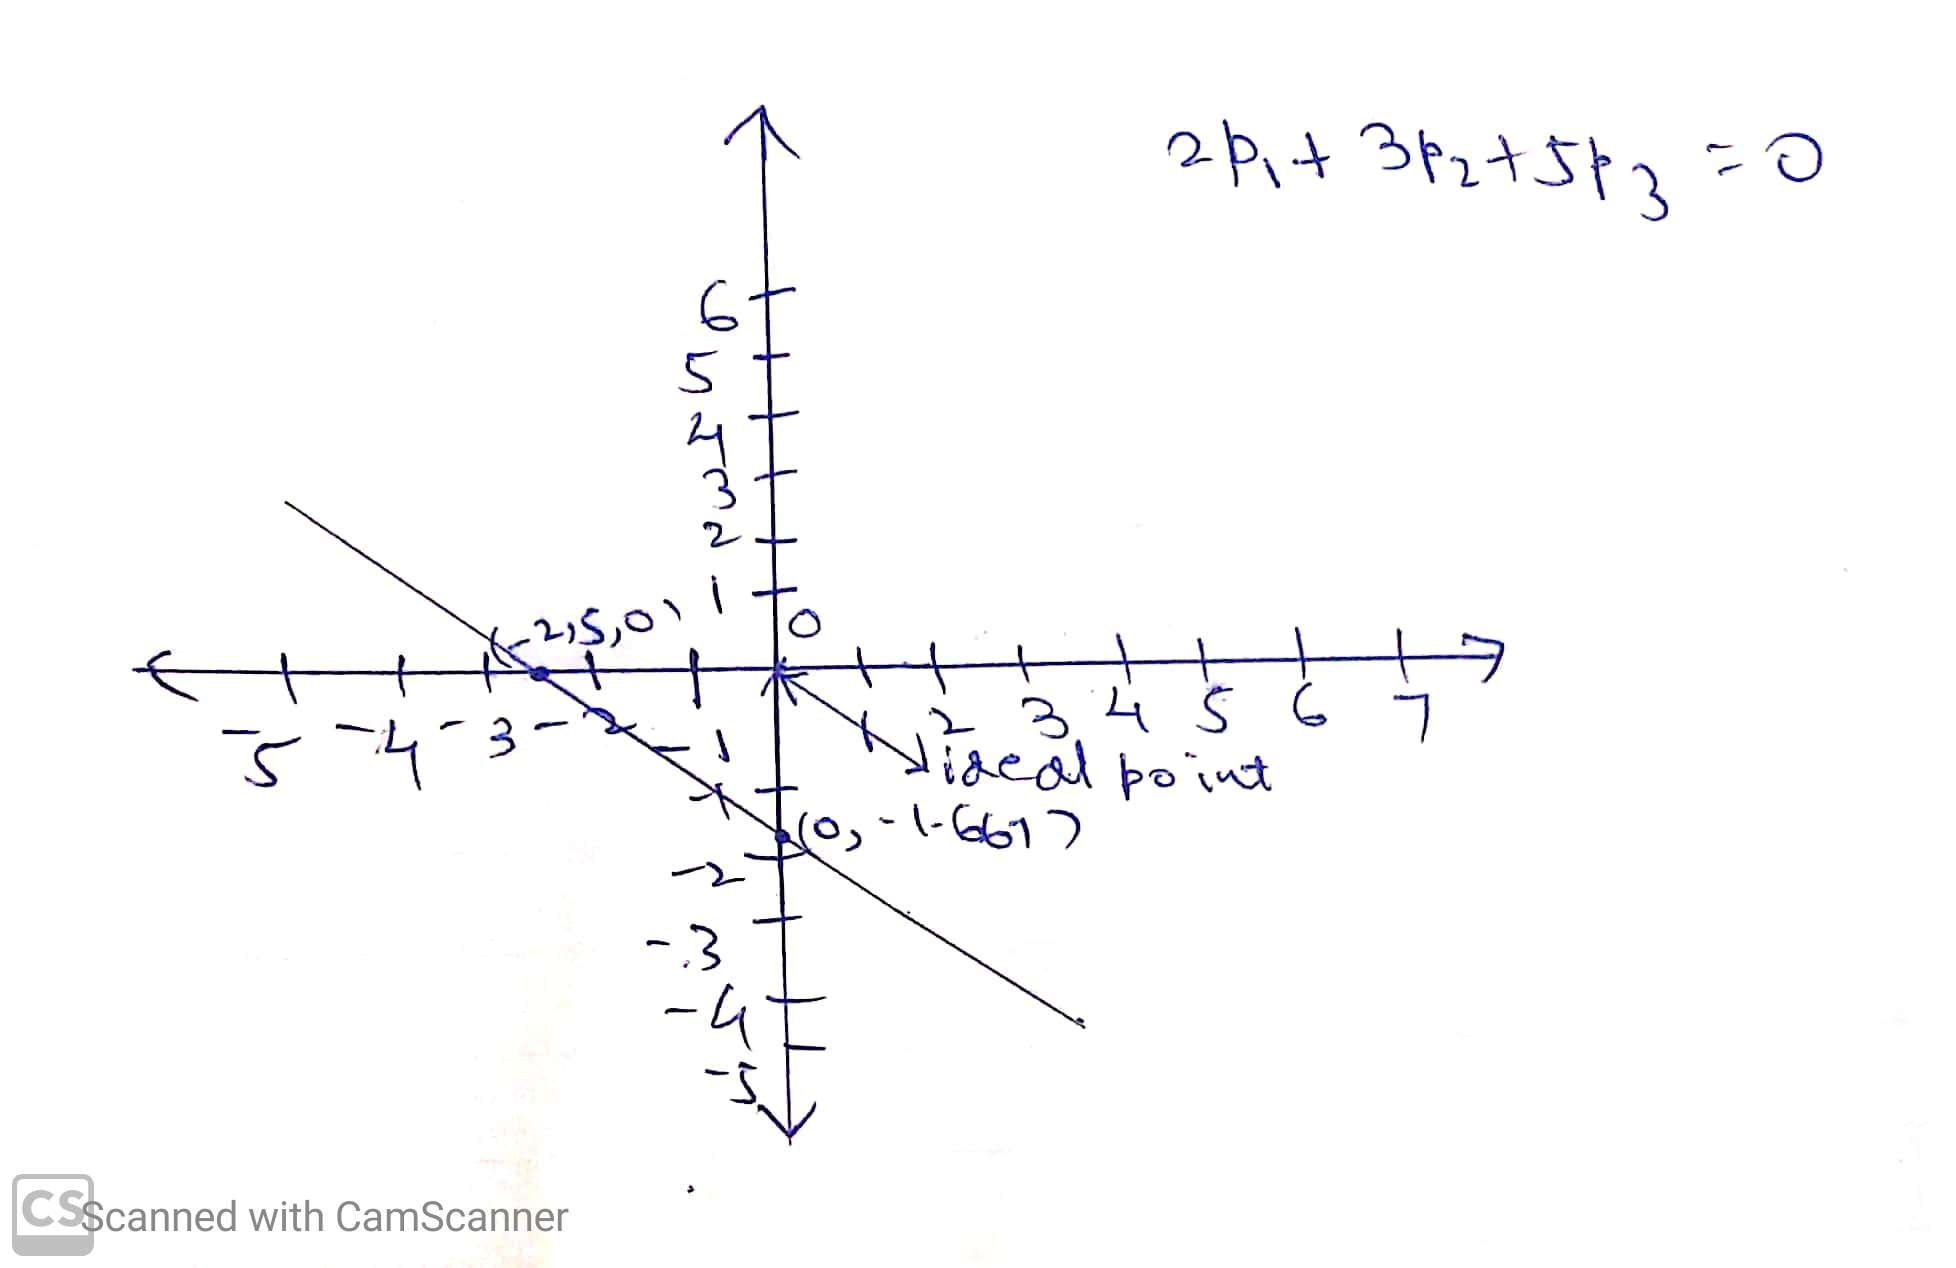
\includegraphics[scale=.15]{61}\\
    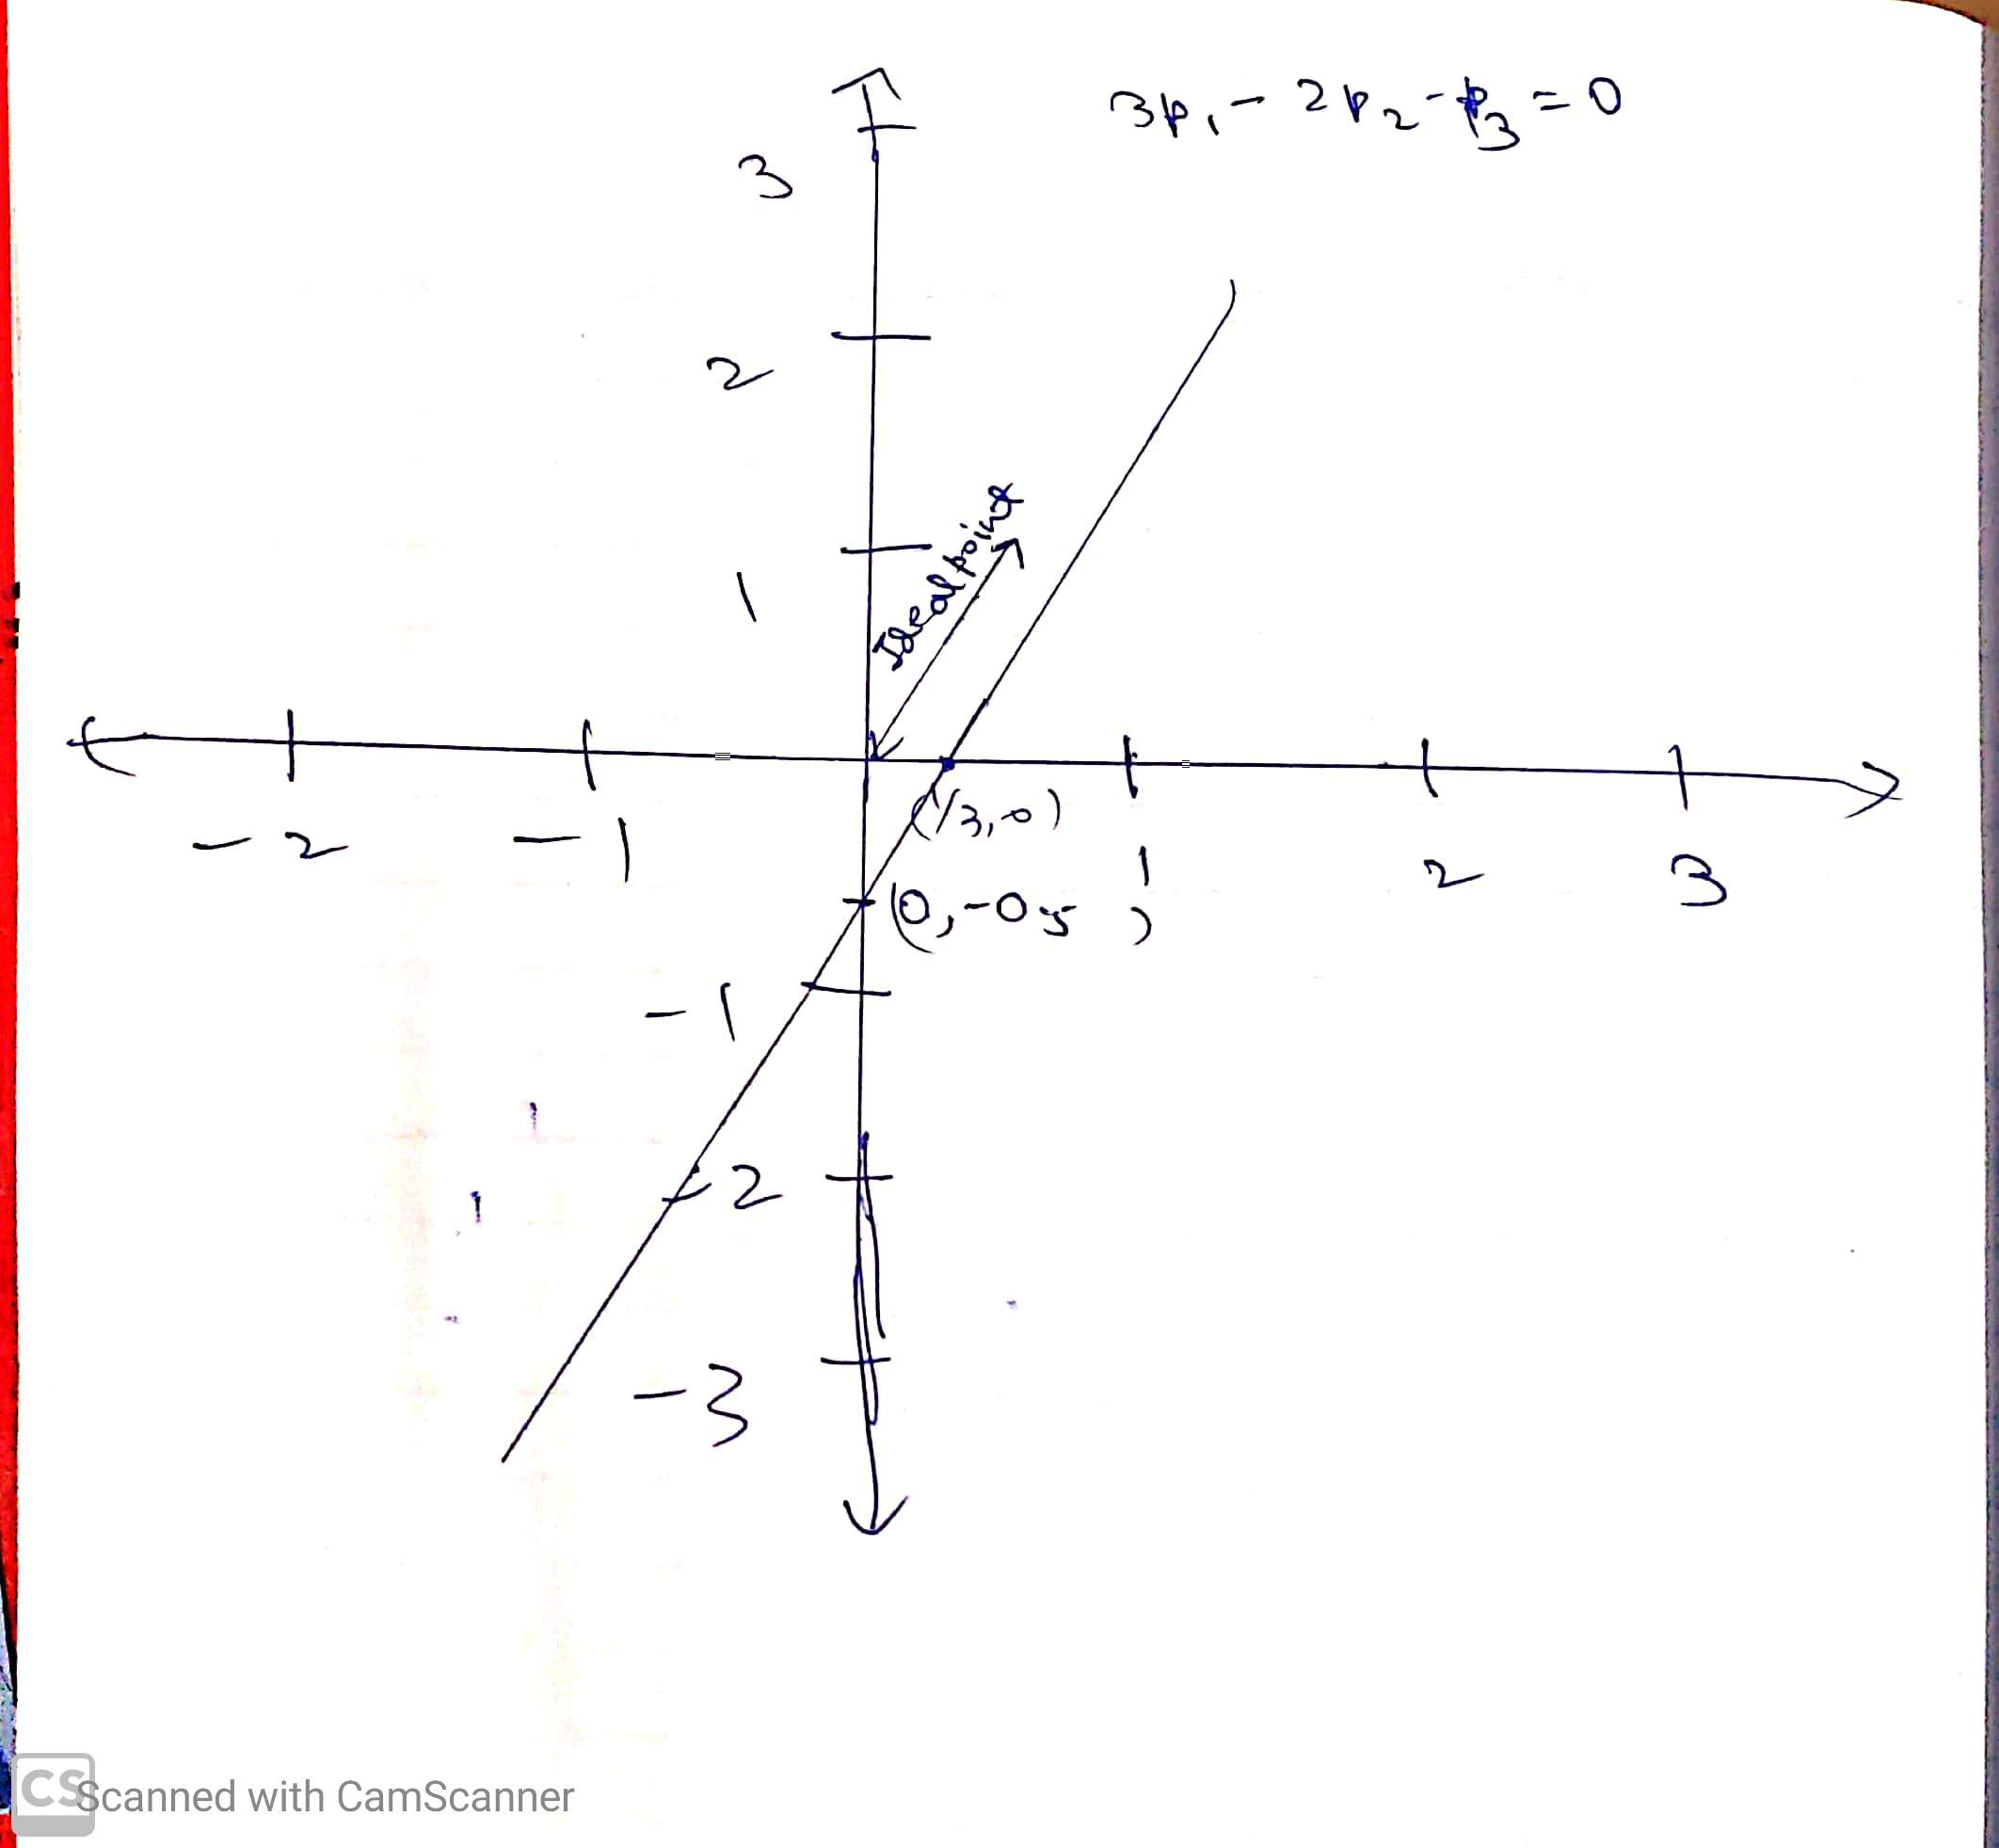
\includegraphics[scale=.15]{62}
    \label{fig:my_label}
\end{figure}
\vspace{1cm}

\end{studentSpace}


\end{tcolorbox} \begin{tcolorbox}
\item  In each of the following cases, sketch the line determined by the two given points; then find the equation of the line.
\begin{multicols}{2}
\begin{enumerate}[]
\item
$A[3, 1, 2]$, $B[1,2,-1]$
\item
$A[2,1,3]$, $B[1,2,0]$
\end{enumerate}
\end{multicols}
\begin{studentSpace}
\begin{figure}[H]
    \centering
    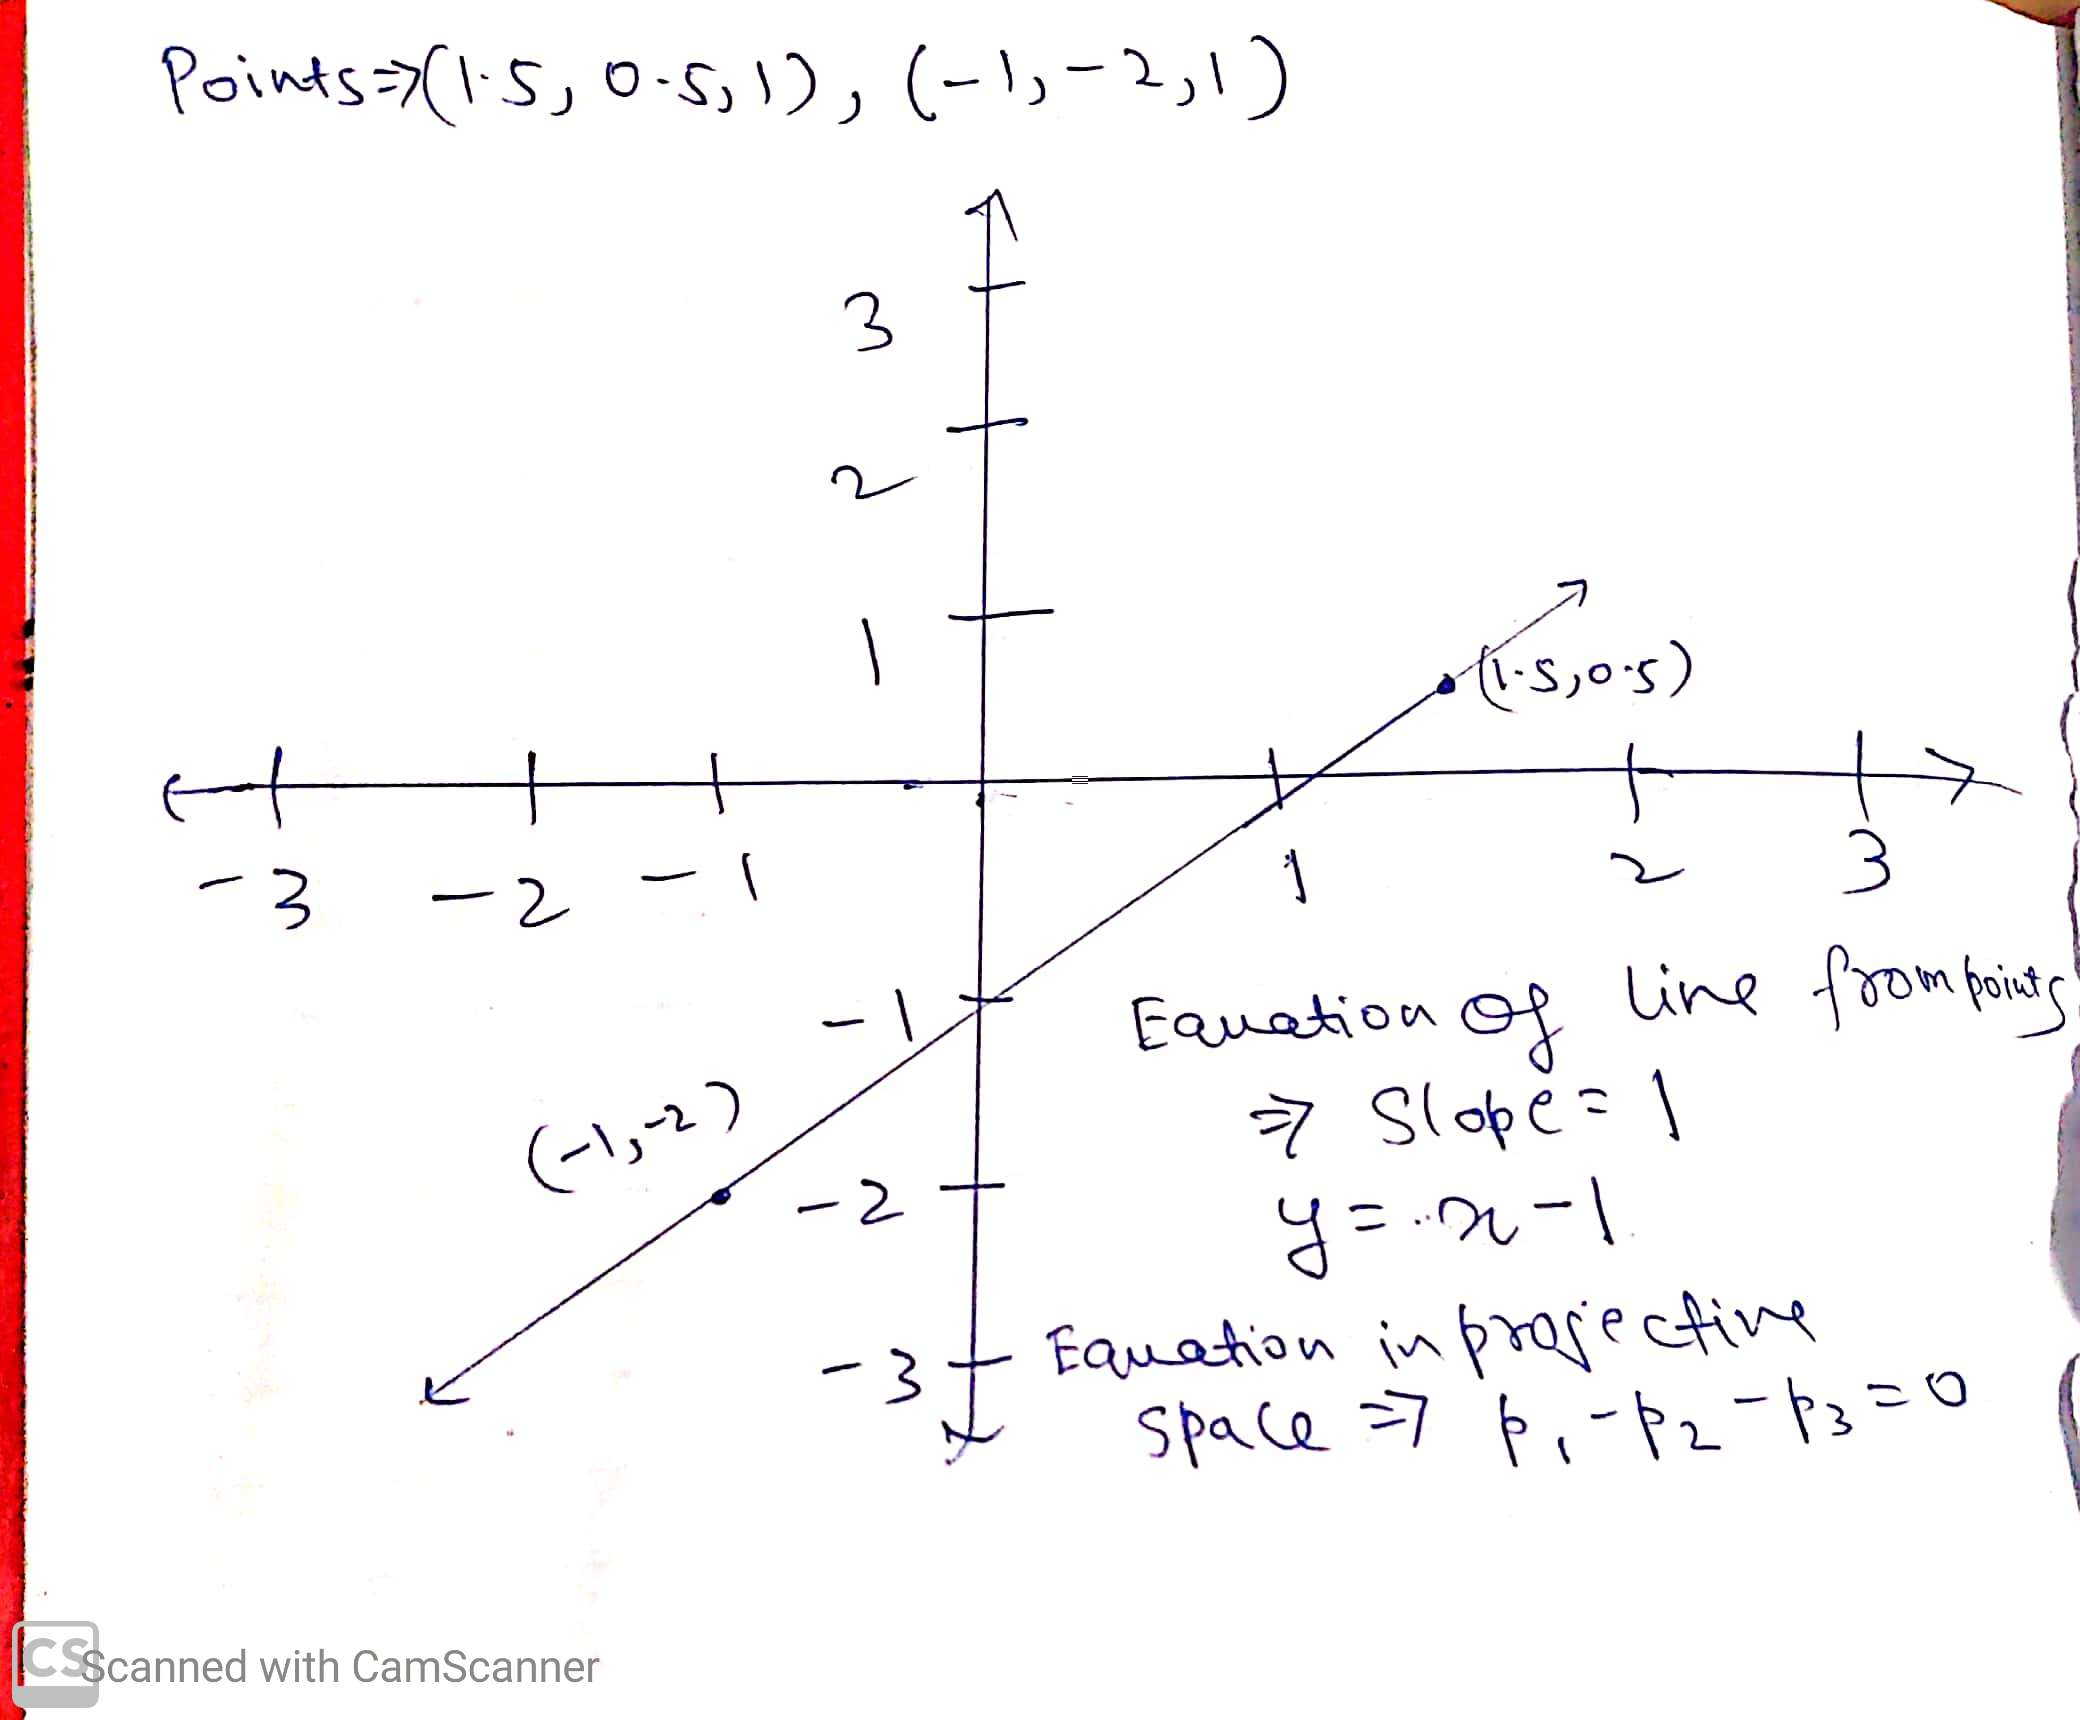
\includegraphics[scale=.15]{71}\\
    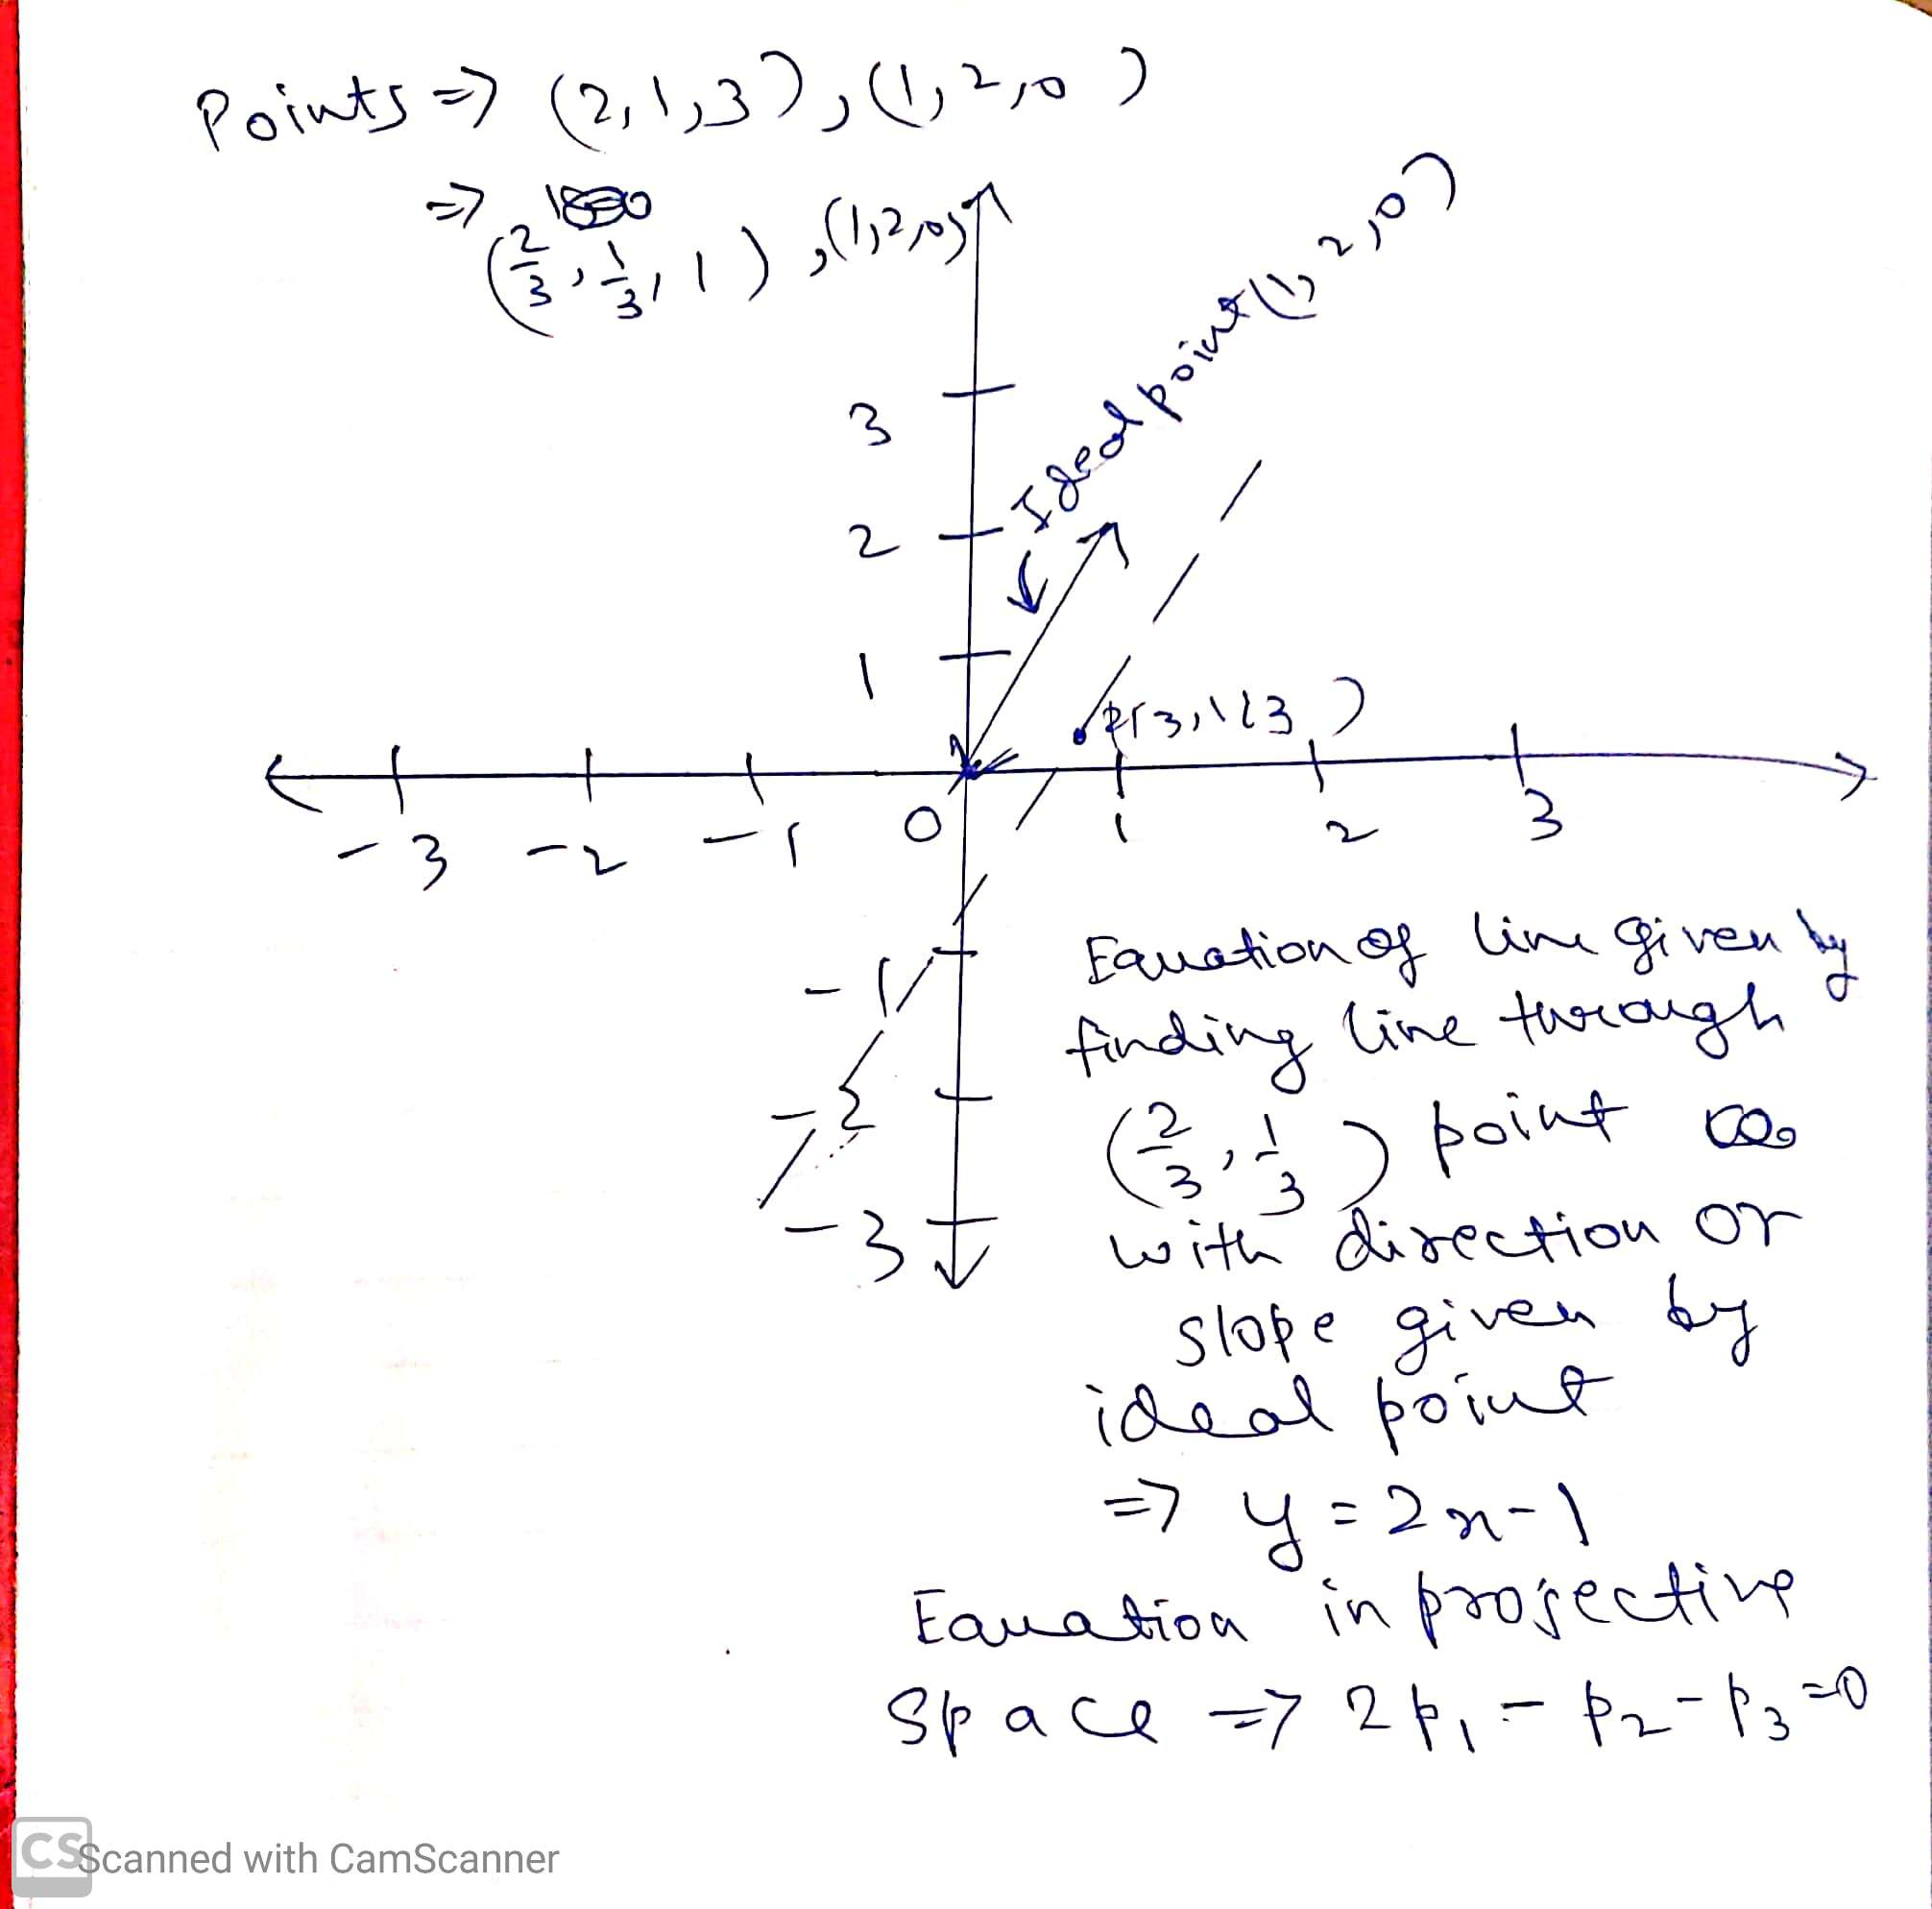
\includegraphics[scale=.15]{72}
    \label{fig:my_label}
\end{figure}
\vspace{1cm}
\end{studentSpace}


\end{tcolorbox} \begin{tcolorbox}
\item  Find the standard homogeneous coordinates of the point of
  intersection for each pair of lines. 
\begin{multicols}{2}
\begin{enumerate}[]
\item
$p_1 + p_2 - 2p_3 = 0, 3p_1 + p_2 + 4p_3 = 0$
\item
$p_1 + p_2 = 0, 4p_1 - 2p_2 + p_3 = 0$
\end{enumerate}
\end{multicols}
\begin{studentSpace}
Ans\\
The point of intersection of 2 lines is given by their cross product in projective space. Hence:\\
a)(1,1,-2)$\times$(3,1,4) = (6,-10,-2) = (-3,5,1). Hence point of intersection of these 2 lines is (-3,5,1)\\
b) (1,1,0)$\times$(4,-2,1) = (1,-1,-6) = $(\frac{-1}{6},\frac{1}{6},1)$. Hence point of intersection of these 2 lines is $(\frac{-1}{6},\frac{1}{6},1)$
\vspace{1cm}
\end{studentSpace}


\end{tcolorbox} \begin{tcolorbox}
\item  Determine which of the following sets of three points are collinear. 
\begin{multicols}{2}
\begin{enumerate}[]
\item
$A[1,2,1]$, $B[0,1,3]$, $[2,1,1]$
\item
$A[1,2,3]$, $B[2,4,3]$, $[1,2,-2]$
\end{enumerate}
\end{multicols}
\begin{studentSpace}
Ans\\
The collinearity of 3 points can be checked simply by finding the determinant formed by the 3 points. If it is equal to 0, then 3 points are collinear\\
a)
\begin{vmatrix}
1 & 2 & 1 \\ 
0 & 1 & 3 \\ 
2 & 1 & 1
\end{vmatrix}
= 8\notag\\
Since the determinant value is not equal to 0, hence the three points are not collinear.\\\\
b)
\begin{vmatrix}
1 & 2 & 3 \\ 
2 & 4 & 3 \\ 
1 & 2 & -2
\end{vmatrix}
= 0\notag\\
Since the determinant value is equal to 0, hence the three points are collinear.\\
\vspace{1cm}
\end{studentSpace}

\end{tcolorbox} \begin{tcolorbox}
\item  Determine which of the following sets of three lines meet in a
  point. 
\begin{multicols}{2}
\begin{enumerate}[]
\item
$l[1,0,1], m[1,1,0], n[0,1,-1]$
\item
$l[1,0,-1], m[1,-2,1], n[3,-2,-1]$
\end{enumerate}
\end{multicols}
\begin{studentSpace}
Ans\\
To find the point of intersection of 3 lines, we simply compute the determinant formed by the coordinates of lines. If that is equal to 0, then three lines meet in a point.\\
a) a)
\begin{vmatrix}
1 & 0 & 1 \\ 
1 & 1 & 0 \\ 
0 & 1 & -1
\end{vmatrix}
= 0\notag\\
Since the determinant value is  equal to 0, hence the three lines meet in a point\\\\
b)
\begin{vmatrix}
1 & 0 & -1 \\ 
1 & -2 & 1 \\ 
3 & -2 & -1
\end{vmatrix}
= 0\notag\\
Since the determinant value is  equal to 0, hence the three lines  meet in a point.\\
\vspace{1cm}
\end{studentSpace}
\end{tcolorbox}

\end{enumerate}
\end{document}

